\documentclass[border=10pt]{standalone}
\usepackage{tikz}
\definecolor{myred}{RGB}{190,60,45}
\definecolor{myblue}{RGB}{38,84,160}
\begin{document}
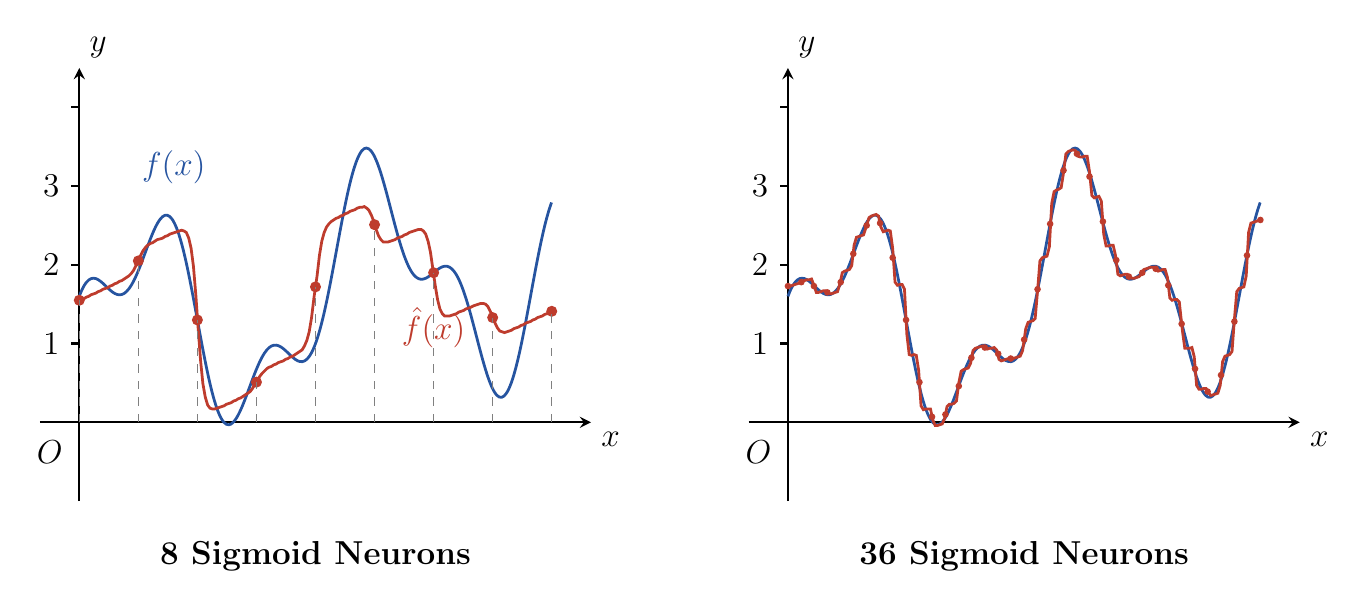
\begin{tikzpicture}[>=stealth, line width=0.8pt, font=\large,
    declare function={f(\x) = 1.2*sin(\x*120) + 0.6*cos(\x*300) + 0.2*\x + 1;}]

  % ===== 左：8 个隐含神经元（欠拟合）=====
  \begin{scope}[xshift=0cm]
    \draw[->] (-0.5,0) -- (6.5,0)   node[below right] {$x$};
    \draw[->] (0,-1.0) -- (0,4.5)   node[above right] {$y$};
    \coordinate (origin) at (0,0);
    \foreach \t in {1,2,3,4} \draw (0,\t) -- ++(-0.1,0);
    \foreach \t in {1,2,3}   \node[left] at (-0.12,\t) {$\t$};
    \node[below left] at (-0.08,-0.1) {$O$};
    \draw[myblue, line width=1pt, smooth, samples=200, domain=0:6]
      plot (\x, {f(\x)});
    \node[myblue] at (1.2,{f(1.2)+0.7}) {$f(x)$};
    \draw[myred, line width=1pt] plot coordinates {(0.00,1.55) (0.03,1.56) (0.06,1.57) (0.09,1.59) (0.12,1.60) (0.15,1.62) (0.18,1.63) (0.21,1.64) (0.24,1.66) (0.27,1.67) (0.30,1.69) (0.33,1.70) (0.36,1.71) (0.39,1.73) (0.42,1.74) (0.45,1.76) (0.48,1.77) (0.51,1.79) (0.54,1.80) (0.57,1.82) (0.60,1.84) (0.63,1.86) (0.66,1.89) (0.69,1.93) (0.72,1.99) (0.75,2.06) (0.78,2.12) (0.81,2.18) (0.84,2.22) (0.87,2.25) (0.90,2.27) (0.93,2.28) (0.96,2.30) (0.99,2.32) (1.03,2.33) (1.06,2.34) (1.09,2.36) (1.12,2.37) (1.15,2.39) (1.18,2.40) (1.21,2.41) (1.24,2.42) (1.27,2.43) (1.30,2.44) (1.33,2.43) (1.36,2.41) (1.39,2.34) (1.42,2.21) (1.45,1.98) (1.48,1.62) (1.51,1.19) (1.54,0.79) (1.57,0.49) (1.60,0.32) (1.63,0.22) (1.66,0.18) (1.69,0.17) (1.72,0.17) (1.75,0.18) (1.78,0.19) (1.81,0.20) (1.84,0.21) (1.87,0.23) (1.90,0.24) (1.93,0.25) (1.96,0.27) (1.99,0.28) (2.02,0.30) (2.05,0.31) (2.08,0.33) (2.11,0.35) (2.14,0.37) (2.17,0.39) (2.20,0.43) (2.23,0.48) (2.26,0.53) (2.29,0.58) (2.32,0.62) (2.35,0.65) (2.38,0.68) (2.41,0.70) (2.44,0.71) (2.47,0.73) (2.50,0.74) (2.53,0.76) (2.56,0.77) (2.59,0.78) (2.62,0.80) (2.65,0.81) (2.68,0.83) (2.71,0.84) (2.74,0.86) (2.77,0.88) (2.80,0.90) (2.83,0.92) (2.86,0.97) (2.89,1.04) (2.92,1.15) (2.95,1.33) (2.98,1.58) (3.02,1.86) (3.05,2.12) (3.08,2.30) (3.11,2.41) (3.14,2.48) (3.17,2.52) (3.20,2.55) (3.23,2.57) (3.26,2.59) (3.29,2.60) (3.32,2.62) (3.35,2.63) (3.38,2.65) (3.41,2.66) (3.44,2.68) (3.47,2.69) (3.50,2.70) (3.53,2.72) (3.56,2.73) (3.59,2.73) (3.62,2.74) (3.65,2.72) (3.68,2.69) (3.71,2.63) (3.74,2.55) (3.77,2.45) (3.80,2.37) (3.83,2.32) (3.86,2.29) (3.89,2.29) (3.92,2.29) (3.95,2.30) (3.98,2.31) (4.01,2.32) (4.04,2.34) (4.07,2.35) (4.10,2.36) (4.13,2.38) (4.16,2.39) (4.19,2.41) (4.22,2.42) (4.25,2.43) (4.28,2.44) (4.31,2.45) (4.34,2.45) (4.37,2.43) (4.40,2.39) (4.43,2.30) (4.46,2.16) (4.49,1.95) (4.52,1.74) (4.55,1.56) (4.58,1.44) (4.61,1.38) (4.64,1.35) (4.67,1.35) (4.70,1.35) (4.73,1.36) (4.76,1.37) (4.79,1.38) (4.82,1.40) (4.85,1.41) (4.88,1.42) (4.91,1.44) (4.94,1.45) (4.97,1.46) (5.01,1.48) (5.04,1.49) (5.07,1.50) (5.10,1.51) (5.13,1.51) (5.16,1.50) (5.19,1.47) (5.22,1.41) (5.25,1.34) (5.28,1.26) (5.31,1.20) (5.34,1.16) (5.37,1.15) (5.40,1.14) (5.43,1.15) (5.46,1.16) (5.49,1.17) (5.52,1.19) (5.55,1.20) (5.58,1.21) (5.61,1.23) (5.64,1.24) (5.67,1.26) (5.70,1.27) (5.73,1.28) (5.76,1.30) (5.79,1.31) (5.82,1.33) (5.85,1.34) (5.88,1.35) (5.91,1.37) (5.94,1.38) (5.97,1.40) (6.00,1.41)};
    \node[myred] at (4.5,1.20) {$\hat{f}(x)$};
    \fill[myred] (0.00,1.55) circle (2pt); \draw[gray, dashed, line width=0.5pt] (0.00,0) -- (0.00,1.55);
    \fill[myred] (0.75,2.05) circle (2pt); \draw[gray, dashed, line width=0.5pt] (0.75,0) -- (0.75,2.05);
    \fill[myred] (1.50,1.30) circle (2pt); \draw[gray, dashed, line width=0.5pt] (1.50,0) -- (1.50,1.30);
    \fill[myred] (2.25,0.51) circle (2pt); \draw[gray, dashed, line width=0.5pt] (2.25,0) -- (2.25,0.51);
    \fill[myred] (3.00,1.72) circle (2pt); \draw[gray, dashed, line width=0.5pt] (3.00,0) -- (3.00,1.72);
    \fill[myred] (3.75,2.51) circle (2pt); \draw[gray, dashed, line width=0.5pt] (3.75,0) -- (3.75,2.51);
    \fill[myred] (4.50,1.90) circle (2pt); \draw[gray, dashed, line width=0.5pt] (4.50,0) -- (4.50,1.90);
    \fill[myred] (5.25,1.33) circle (2pt); \draw[gray, dashed, line width=0.5pt] (5.25,0) -- (5.25,1.33);
    \fill[myred] (6.00,1.41) circle (2pt); \draw[gray, dashed, line width=0.5pt] (6.00,0) -- (6.00,1.41);
    \node[font=\large\bfseries] at (3,-1.7) {8 Sigmoid Neurons};
  \end{scope}

  % ===== 右：36 个隐含神经元（万能逼近）=====
  \begin{scope}[xshift=9cm]
    \draw[->] (-0.5,0) -- (6.5,0)   node[below right] {$x$};
    \draw[->] (0,-1.0) -- (0,4.5)   node[above right] {$y$};
    \coordinate (origin) at (0,0);
    \foreach \t in {1,2,3,4} \draw (0,\t) -- ++(-0.1,0);
    \foreach \t in {1,2,3}   \node[left] at (-0.12,\t) {$\t$};
    \node[below left] at (-0.08,-0.1) {$O$};
    \draw[myblue, line width=1pt, smooth, samples=200, domain=0:6]
      plot (\x, {f(\x)});
    \draw[myred, line width=1pt] plot coordinates {(0.00,1.73) (0.03,1.73) (0.06,1.74) (0.09,1.75) (0.12,1.76) (0.15,1.77) (0.18,1.79) (0.21,1.80) (0.24,1.81) (0.27,1.81) (0.30,1.82) (0.33,1.74) (0.36,1.65) (0.39,1.65) (0.42,1.66) (0.45,1.67) (0.48,1.67) (0.51,1.64) (0.54,1.63) (0.57,1.64) (0.60,1.65) (0.63,1.66) (0.66,1.76) (0.69,1.90) (0.72,1.92) (0.75,1.93) (0.78,1.94) (0.81,1.99) (0.84,2.25) (0.87,2.35) (0.90,2.36) (0.93,2.37) (0.96,2.38) (0.99,2.47) (1.03,2.60) (1.06,2.62) (1.09,2.63) (1.12,2.64) (1.15,2.62) (1.18,2.48) (1.21,2.42) (1.24,2.43) (1.27,2.44) (1.30,2.43) (1.33,2.21) (1.36,1.78) (1.39,1.74) (1.42,1.75) (1.45,1.75) (1.48,1.69) (1.51,1.12) (1.54,0.86) (1.57,0.85) (1.60,0.86) (1.63,0.85) (1.66,0.66) (1.69,0.21) (1.72,0.16) (1.75,0.17) (1.78,0.17) (1.81,0.17) (1.84,0.03) (1.87,-0.04) (1.90,-0.04) (1.93,-0.03) (1.96,-0.02) (1.99,0.05) (2.02,0.20) (2.05,0.23) (2.08,0.23) (2.11,0.24) (2.14,0.27) (2.17,0.50) (2.20,0.65) (2.23,0.67) (2.26,0.68) (2.29,0.69) (2.32,0.75) (2.35,0.91) (2.38,0.94) (2.41,0.95) (2.44,0.96) (2.47,0.97) (2.50,0.95) (2.53,0.93) (2.56,0.94) (2.59,0.94) (2.62,0.95) (2.65,0.92) (2.68,0.80) (2.71,0.78) (2.74,0.79) (2.77,0.80) (2.80,0.81) (2.83,0.81) (2.86,0.81) (2.89,0.82) (2.92,0.83) (2.95,0.84) (2.98,0.91) (3.02,1.19) (3.05,1.27) (3.08,1.28) (3.11,1.29) (3.14,1.32) (3.17,1.67) (3.20,2.05) (3.23,2.09) (3.26,2.10) (3.29,2.11) (3.32,2.23) (3.35,2.78) (3.38,2.93) (3.41,2.95) (3.44,2.96) (3.47,2.98) (3.50,3.17) (3.53,3.41) (3.56,3.44) (3.59,3.45) (3.62,3.46) (3.65,3.45) (3.68,3.38) (3.71,3.37) (3.74,3.37) (3.77,3.38) (3.80,3.38) (3.83,3.18) (3.86,2.88) (3.89,2.85) (3.92,2.86) (3.95,2.87) (3.98,2.81) (4.01,2.39) (4.04,2.24) (4.07,2.24) (4.10,2.25) (4.13,2.25) (4.16,2.12) (4.19,1.88) (4.22,1.86) (4.25,1.87) (4.28,1.88) (4.31,1.88) (4.34,1.84) (4.37,1.83) (4.40,1.83) (4.43,1.84) (4.46,1.85) (4.49,1.88) (4.52,1.94) (4.55,1.95) (4.58,1.96) (4.61,1.97) (4.64,1.97) (4.67,1.94) (4.70,1.92) (4.73,1.93) (4.76,1.94) (4.79,1.94) (4.82,1.84) (4.85,1.58) (4.88,1.55) (4.91,1.56) (4.94,1.56) (4.97,1.53) (5.01,1.16) (5.04,0.94) (5.07,0.94) (5.10,0.94) (5.13,0.95) (5.16,0.83) (5.19,0.47) (5.22,0.42) (5.25,0.42) (5.28,0.43) (5.31,0.43) (5.34,0.38) (5.37,0.34) (5.40,0.35) (5.43,0.36) (5.46,0.37) (5.49,0.47) (5.52,0.77) (5.55,0.84) (5.58,0.85) (5.61,0.86) (5.64,0.90) (5.67,1.31) (5.70,1.66) (5.73,1.70) (5.76,1.71) (5.79,1.72) (5.82,1.86) (5.85,2.41) (5.88,2.53) (5.91,2.54) (5.94,2.55) (5.97,2.56) (6.00,2.57)};
    \fill[myred] (0.00,1.73) circle (1.2pt);
    \fill[myred] (0.17,1.78) circle (1.2pt);
    \fill[myred] (0.33,1.73) circle (1.2pt);
    \fill[myred] (0.50,1.65) circle (1.2pt);
    \fill[myred] (0.67,1.78) circle (1.2pt);
    \fill[myred] (0.83,2.14) circle (1.2pt);
    \fill[myred] (1.00,2.50) circle (1.2pt);
    \fill[myred] (1.17,2.53) circle (1.2pt);
    \fill[myred] (1.33,2.09) circle (1.2pt);
    \fill[myred] (1.50,1.30) circle (1.2pt);
    \fill[myred] (1.67,0.51) circle (1.2pt);
    \fill[myred] (1.83,0.07) circle (1.2pt);
    \fill[myred] (2.00,0.10) circle (1.2pt);
    \fill[myred] (2.17,0.46) circle (1.2pt);
    \fill[myred] (2.33,0.82) circle (1.2pt);
    \fill[myred] (2.50,0.95) circle (1.2pt);
    \fill[myred] (2.67,0.87) circle (1.2pt);
    \fill[myred] (2.83,0.81) circle (1.2pt);
    \fill[myred] (3.00,1.05) circle (1.2pt);
    \fill[myred] (3.17,1.69) circle (1.2pt);
    \fill[myred] (3.33,2.52) circle (1.2pt);
    \fill[myred] (3.50,3.20) circle (1.2pt);
    \fill[myred] (3.67,3.41) circle (1.2pt);
    \fill[myred] (3.83,3.12) circle (1.2pt);
    \fill[myred] (4.00,2.55) circle (1.2pt);
    \fill[myred] (4.17,2.06) circle (1.2pt);
    \fill[myred] (4.33,1.85) circle (1.2pt);
    \fill[myred] (4.50,1.90) circle (1.2pt);
    \fill[myred] (4.67,1.95) circle (1.2pt);
    \fill[myred] (4.83,1.74) circle (1.2pt);
    \fill[myred] (5.00,1.25) circle (1.2pt);
    \fill[myred] (5.17,0.68) circle (1.2pt);
    \fill[myred] (5.33,0.39) circle (1.2pt);
    \fill[myred] (5.50,0.60) circle (1.2pt);
    \fill[myred] (5.67,1.28) circle (1.2pt);
    \fill[myred] (5.83,2.12) circle (1.2pt);
    \fill[myred] (6.00,2.57) circle (1.2pt);
    \node[font=\large\bfseries] at (3,-1.7) {36 Sigmoid Neurons};
  \end{scope}

\end{tikzpicture}
\end{document}
